\apendice{Documentación de usuario}

\section{Introducción}

En este anexo se pretende describir de forma concisa las características y funcionalidades de la \textit{web} desarrollada, además de los requisitos necesarios para su correcta renderización.

Es importante destacar que la \textit{web} ha sido desplegada en Heroku. Sin embargo, esta PaaS, tiene importantes restricciones en las versiones para estudiantes. En concreto, Krini se ve gravemente perjudicada ya que Heroku cancela toda petición que dure más de 30 segundos (lo que impide, en la mayoría de los enlaces, realizar un análisis completo).

Por este motivo, también se va a documentar cómo desplegar la aplicación en local (servidor de producción y base de datos) mediante contenedores de Docker.

\section{Requisitos de usuarios}

En este apartado se pretenden enumerar los requisitos necesarios para acceder correctamente a la \textit{web} desarrollada.

\subsection{Requisitos Heroku}
\label{s-e:requisitos-heroku}

Los requisitos en este caso vienen limitados por el uso de las bibliotecas \texttt{Chart.js} (v2.9.3) y \texttt{Bootstrap} (v4.4.1). En este caso, se necesita que la \textit{web} se renderice en navegadores con las siguientes versiones:

\begin{itemize}
	\item \textbf{Google Chrome:} todas las versiones modernas.
	\item \textbf{Mozilla Firefox:} todas las versiones modernas.
	\item \textbf{Safari:} todas las versiones modernas.
	\item \textbf{Microsoft Edge:} todas las versiones modernas.
	\item \textbf{Internet Explorer:} versión 10 o superior.
\end{itemize}

\subsection{Requisitos Docker}
\label{s-e:requisitos-docker}

Además de los requisitos expuestos en la sección~\ref{s-e:requisitos-heroku}, si se quiere ejecutar el contenedor de Docker en local, se ha de cumplir con las siguientes características en función del sistema operativo. Es relevante que, como se puede comprobar en el diagrama de despliegue de Docker (disponible en la ilustración~\ref{c:diagrama-deploy-docker}), los contenedores de la base de datos y de la \textit{web} son independientes. Por ello, se ha de contar con el \textit{plugin} \texttt{docker-compose}.

\begin{enumerate}
	\item \textbf{Windows}: se recomienda utilizar Docker Desktop por su simplicidad. Los requisitos completos se pueden consultar en su documentación oficial\footnote{Disponible en \url{https://docs.docker.com/desktop/install/windows-install/}}. Sin embargo, se resumen a continuación:
	
	\begin{itemize}
		\item \texttt{WLS}
		\item Procesador de 64 bits
		\item 4GB de memoria RAM
		\item 3GB de memoria para las imágenes
		\item El \textit{plugin} \texttt{docker-compose} viene por defecto con la versión de escritorio.
	\end{itemize}

	\item \textbf{Linux}: nuevamente, los requisitos completos se facilitan en la documentación\footnote{Disponible en \url{https://docs.docker.com/desktop/install/linux-install/}}. En resumen, se recomienda:
	\begin{itemize}
		\item Disponer de soporte para virtualización
		\item Procesador de 64 bits
		\item 4GB de memoria RAM
		\item 3GB de memoria para las imágenes
		\item Instalar el \textit{plugin} \texttt{docker-compose} mediante \texttt{\$ sudo apt-get install docker-compose-plugin} (en Ubuntu y Debian) o \texttt{\$ sudo yum install docker-compose-plugin} (en distribuciones basadas en RPM).
	\end{itemize}
\end{enumerate}



\section{Instalación}

La instalación de un producto \textit{software} es el proceso mediante el cual se configura y prepara un programa o aplicación para que pueda ser utilizado en un dispositivo objetivo.

Debido a que la aplicación desarrollada es una \textit{web}, no hace falta pasar por este proceso. Sin embargo y debido a las restricciones de Heroku anteriormente mencionadas, se va a explicar cómo desplegar la aplicación en local mediante Docker (con servidores de producción) para comprobar la funcionalidad al completo. Se recuerda que las instrucciones para levantar el servidor de desarrollo se encuentran en la sección~\ref{s-d:flask-deploy}.

\subsection{Acceso mediante Heroku}

Simplemente se ha de acceder mediante el navegador introduciendo la dirección \url{https://krini.herokuapp.com/}

\subsection{Despliegue en Docker}
\label{s-e:docker-deploy-users}

Para facilitar que cualquier usuario pueda desplegar un contenedor de Docker (en realidad, dos) y levantar su propio servidor de gunicorn en local sin tener conocimientos técnicos, se han preparado unos \textit{scripts} multiplataforma disponibles en \url{https://github.com/phf1001/semisupervised-learning-in-cibersecurity/tree/main/docker-deploy-kit}

De esta forma, tan solo se debe seleccionar el sistema operativo anfitrión, descargar los archivos (se facilita un comprimido con todos incluidos) y garantizar que se cumple con los requisitos de la sección~\ref{s-e:requisitos-docker}.

Para levantar el servidor en local y garantizar que la base de datos se rellena completamente, se han de seguir los siguientes pasos teniendo en cuenta que los \textit{scripts} en Linux se ejecutan mediante el comando \texttt{\$ sh nombre-script.sh} y en Windows mediante \texttt{\$ nombre-script.bat}.

\begin{enumerate}
	\item Ubicarse en la carpeta donde se encuentren los \textit{scripts}.
	\item Si es la primera vez que se ejecuta:
	\begin{enumerate}
	\item Lanzar el script \texttt{docker-first-time-1.sh} y seguir las instrucciones (esperar 30 segundos y abrir el navegador cuando lo indique).
	\item Ejecutar el \textit{script} \texttt{docker-first-time-2.sh} y respetar los pasos indicados (esperar 30 segundos antes de abrir el navegador).
	\end{enumerate}
	\item Si se quieren parar los contenedores para reutilizarlos luego, ejecutar el \textit{script} \texttt{docker-stop.sh} y \texttt{docker-start.sh} para volver a iniciarlos.
	\item Si se quieren borrar las imágenes y contenedores del sistema definitivamente, ejecutar el \textit{script} \texttt{docker-clean.sh}
\end{enumerate}

\textbf{Importante}: iniciar el demonio de Docker antes de lanzar los \textit{scripts}. En Windows basta con iniciar la aplicación de escritorio.

\section{Manual del usuario}

En este punto del manual se supone que todos los usuarios tienen acceso a la aplicación, ya sea mediante un contenedor de Docker o Heroku.

A continuación, se procede a ilustrar las funcionalidades básicas de la \textit{web}. Es destacable que no todos los usuarios cuentan con acceso a todas las funcionalidades (consultar diagrama de casos de uso~\ref{b:diagrama-cu}). Por ello, se recomienda probar el producto con una cuenta con permisos de administración.

\subsection{Analizador}

\begin{figure}[h]
	\caption[Manual de usuario: página principal]{Página principal de la aplicación.}
	\centering
	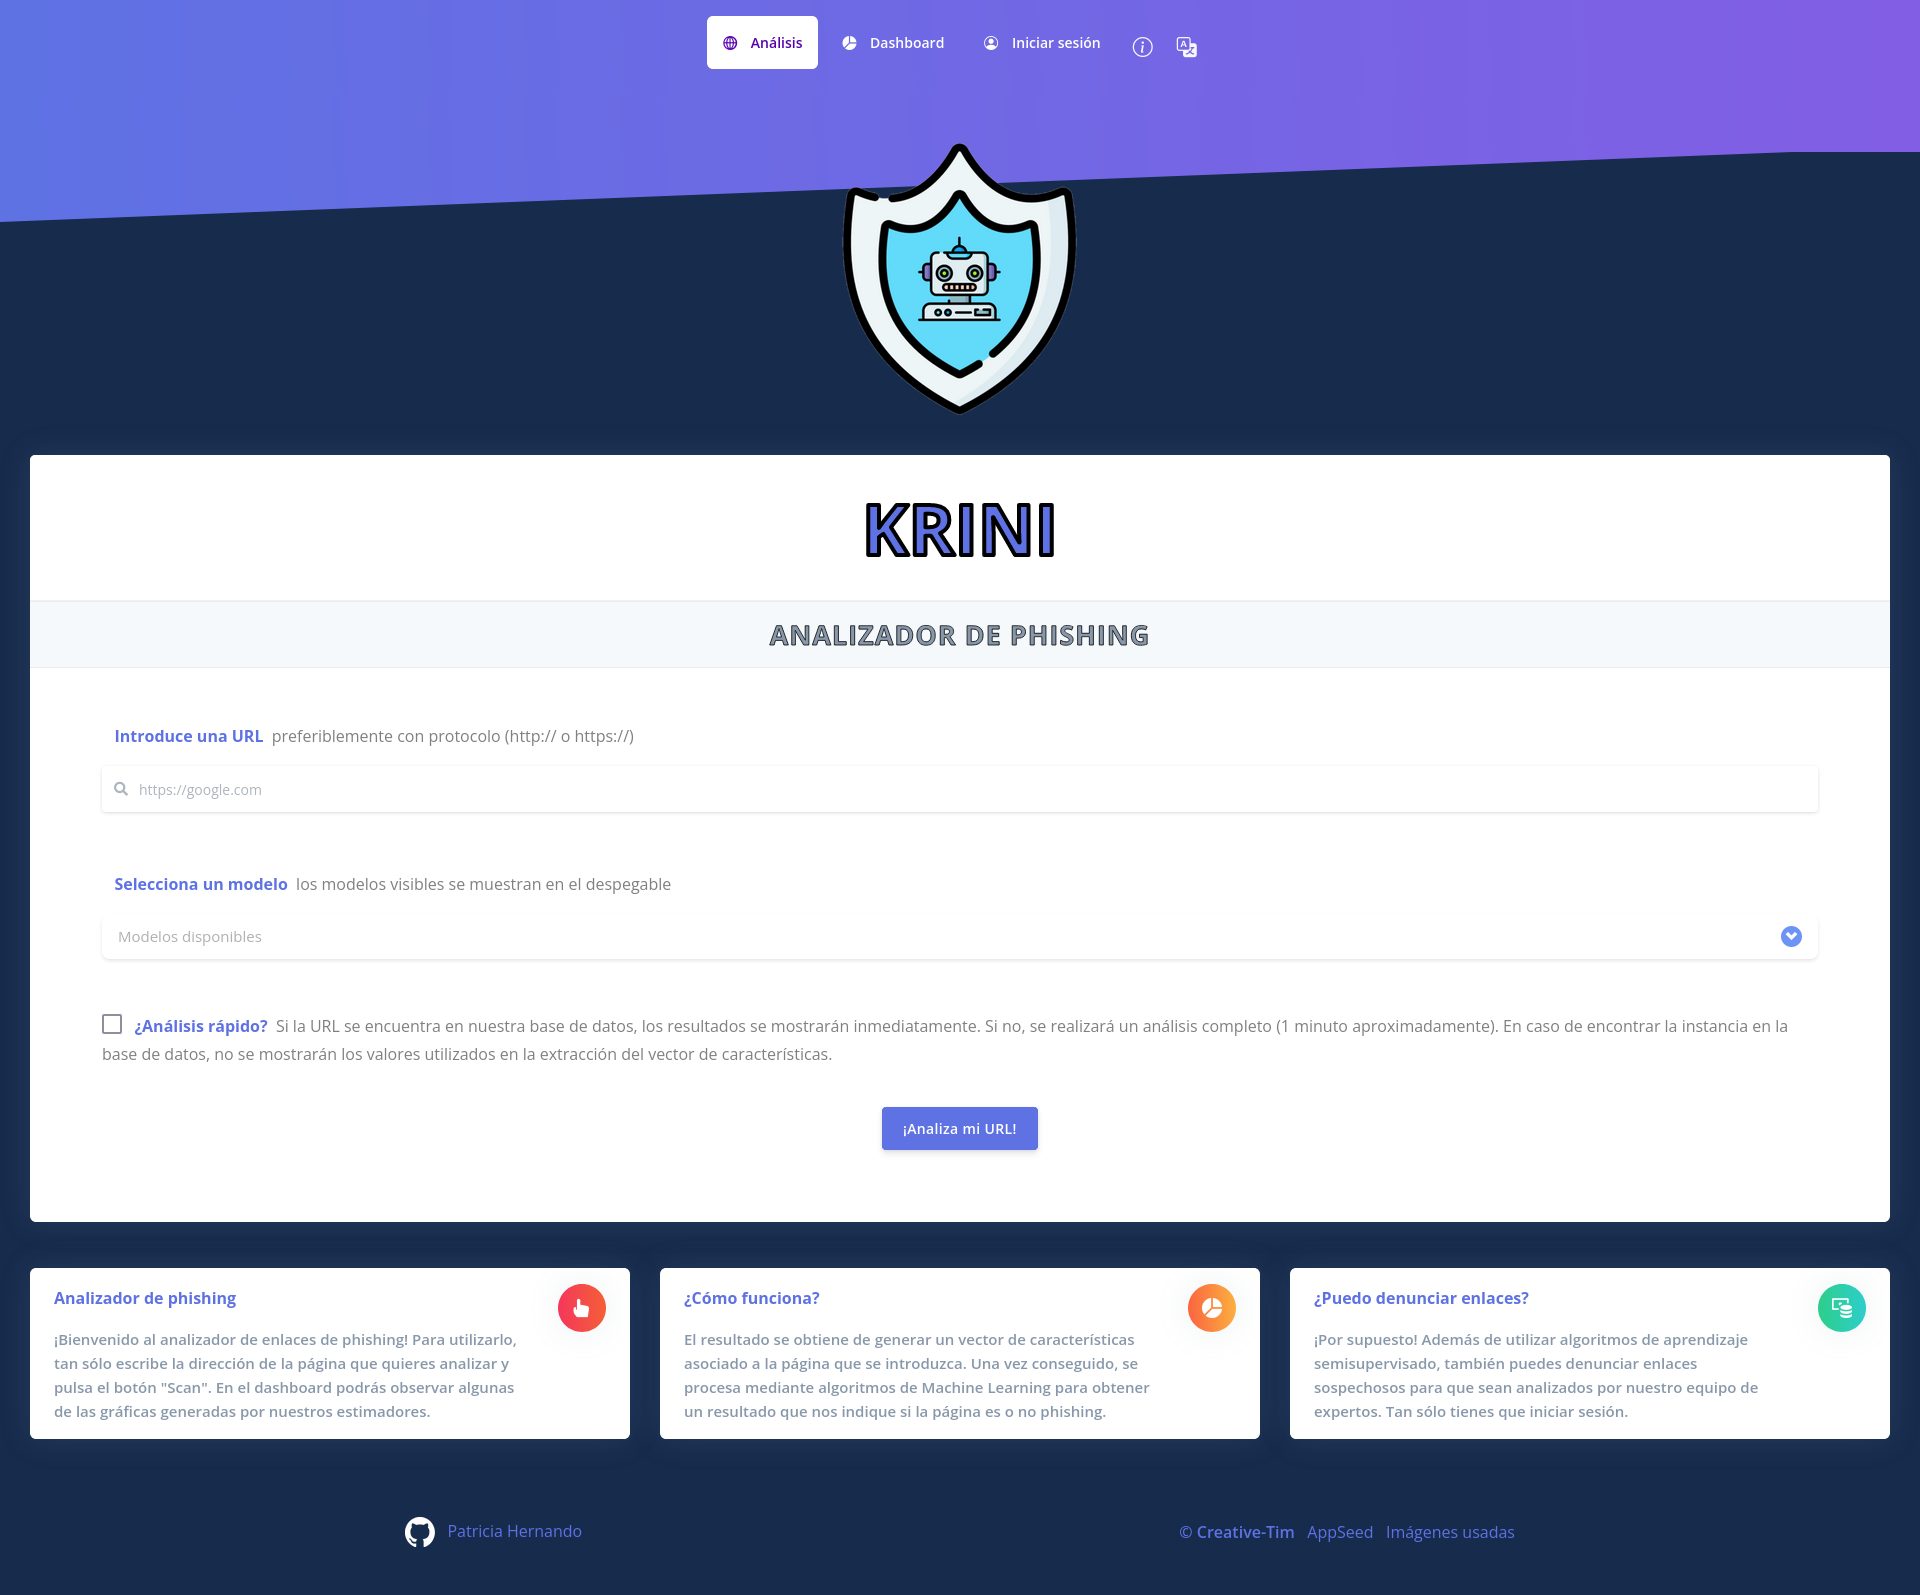
\includegraphics[width=\textwidth]{../img/anexos/user_guide/1_index}
	\label{e-1:index}
\end{figure}
